\themaN
\graphicspath{{../../S17_Distributivite_et_egalites/Images/}}

\chapter{Distributivité simple et égalités}
\label{S17}

\newcommand{\tri}[3]{\pspolygon(0,0)(2,0)(2;60) \rput(1,0.25){$#1$} \rput{-120}(0.7,0.8){$#2$} \rput{120}(1.3,0.8){$#3$}}
\newcommand{\car}[4]{\psframe(0,0)(2,2) \rput(1,0.2){$#1$} \rput{90}(1.8,1){$#2$} \rput{180}(1,1.8){$#3$} \rput{-90}(0.2,1){$#4$}}


%%%%%%%%%%%%%%%%%%%%%%%%%%%%%%
%%%%%%%%%%%%%%%%%%%%%%%%%%%%%%
\begin{autoeval}
   \small
   \begin{enumerate}
      \item Il utilise la distributivité simple pour réduire une expression littérale de la forme $ax + bx$ où $a$ et $b$ sont des nombres décimaux.
      \item Il substitue une valeur numérique à une lettre pour : calculer la valeur d’une expression littérale ; tester, à la main ou de façon instrumentée, si une égalité où figurent une ou deux indéterminées est vraie quand on leur attribue des valeurs numériques ; contrôler son résultat.
   \end{enumerate}
\end{autoeval}

\begin{prerequis}
   \begin{itemize}
      \item Propriétés de distributivité simple.
      \item[\com] Développer, factoriser, réduire des expressions littérales dans des cas très simples.
   \end{itemize}
\end{prerequis}

\vfill

\begin{debat}[Débat : polysémie du facteur]
   La {\bf polysémie} est la caractéristique d'un mot ou d'une expression qui a plusieurs sens ou significations différentes. En mathématiques, on utilise régulièrement des mots qui n'ont pas forcément le même sens qu'en français par exemple. \\
   Le mot {\bf facteur} ne déroge pas à cette règle : étymologiquement, il vient du latin {\it factir}, celui qui fait. Le facteur que nous utilisons en mathématiques désigne un terme d'un produit, et le facteur que nous connaissons le mieux est certainement la personne distribuant le courrier. À l'origine, le facteur est un fabriquant d'instruments de musique. Enfin, le terme facteur s'utilise aussi en économie ou en biologie pour mentionner un élément important qui concourt à un résultat.
   \begin{center}
      \begin{pspicture}(0,0)(3,2)
         \psframe[fillstyle=solid,fillcolor=A1!15](0,0)(3,2)
         \pspolygon[fillstyle=solid,fillcolor=A1!10](0,2)(1.5,0.8)(3,2)
      \end{pspicture}
   \end{center}
   \bigskip
   \begin{cadre}[B2][J4]
      \begin{center}
         Vidéo : \href{https://www.yout-ube.com/watch?v=g73sqrZZlQo}{\bf Comprendre la simple distributivité}, chaîne YouTube de {\it Jean-Yves Labouche}.
      \end{center}
   \end{cadre}
\end{debat}


%%%%%%%%%%%%%%%%%%%%%%%%%%%%%%
%%%%%%%%%%%%%%%%%%%%%%%%%%%%%%
\activites

\begin{activite}[Je veux du chocolat !]
   {\bf Objectifs :} découvrir la distributivité simple pour réduire une expression littérale de la forme $ax+bx$ où $a$ et $b$ sont des nombres décimaux.
   \begin{QCM}
      Un chocolatier expérimente une nouvelle tablette de chocolat pour son magasin : celle-ci est composée de rangées de chocolat dont le cacao vient de côte d'ivoire (CI) et d'un tout nouveau chocolat du Brésil (BR), un peu plus clair. Sa tablette représentée ci-dessous est composée de \ug{64} de chocolat CI et de \ug{32} de chocolat BR.
      \begin{center}
         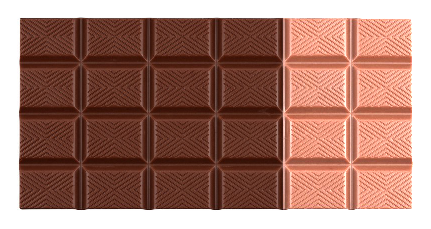
\includegraphics[width=5.25cm]{chocolat}
      \end{center}
      \begin{enumerate}
         \item Il fait un premier test sur 20 tablettes de chocolat qu'il distribue à ses amis pour la tester. \\
            Combien a-t-il besoin de chocolat en tout : trouver deux manières de calculer la masse des 20 tablettes et écrire les deux calculs {\it (aide : on peut utiliser des parenthèses dans l'un des calculs)}. \\ [3mm]
            Calcul 1 : \pointilles \\ [3mm]
            Calcul 2 : \pointilles \bigskip
         \item Ses amis trouvent qu'il n'y a pas de chocolat BR, ils proposent donc un deuxième test sur 35 tablettes de chocolat, mais en utilisant cette fois-ci \ug{56} de chocolat CI et \ug{40} de chocolat BR. \\
            Combien a-t-il besoin de chocolat en tout ? \\ [3mm]
            Calcul 1 : \pointilles \\ [3mm]
            Calcul 2 : \pointilles \bigskip
         \item Pour pouvoir effectuer ses calculs plus rapidement, il décide de trouver une formule littérale qui lui permette de calculer le nombre de carreaux de chocolat dont il aura besoin. \\
         \begin{minipage}{8cm}
            On note :
            \begin{itemize}
               \item $a$ le nombre de rangées de chocolat CI ;
               \item $b$ le nombre de rangées de chocolat BR ;
               \item $x$ le nombre de lignes de chocolat.
            \end{itemize}
         \end{minipage}
         \qquad
         \begin{minipage}{7cm}
            \psset{xunit=0.75,yunit=0.525}
            \begin{pspicture}[subgriddiv=0,gridlabels=0,gridcolor=gray](-3,-0.8)(6,4.8)
               \psgrid(0,0)(6,4)
               \psframe[linewidth=0.5mm](0,0)(6,4)
               \psline[linewidth=0.5mm](4,0)(4,4)
               \psline[linecolor=marron]{<->}(-0.3,0)(-0.3,4)
               \rput(-0.6,1.5){\textcolor{marron}{$x$}}
               \psline[linecolor=marron]{<->}(0,4.4)(4,4.4)
               \rput(2,4.8){\textcolor{marron}{$a$}}
               \psline[linecolor=marron]{<->}(4,4.4)(6,4.4)
                \rput(5,4.8){\textcolor{marron}{$b$}}
            \end{pspicture}
         \end{minipage}
         \begin{enumerate}
            \item Donner deux expressions littérales permettant de calculer le nombre total de carreaux de chocolat. \\ [3mm]
               Calcul 1 : \pointilles \\ [3mm]
               Calcul 2 : \pointilles \bigskip
            \item Sachant que le nombre de carreaux est le même dans les deux expressions, écrire l'égalité qui résulte de ces deux calculs. \\
               \pointilles
         \end{enumerate}
      \end{enumerate}
   \end{QCM}
\end{activite}


%%%%%%%%%%%%%%%%%%%%%%%%%%%%%%
%%%%%%%%%%%%%%%%%%%%%%%%%%%%%%
\cours 

%%%%%%%%%%%%%%%%%%%%%%%
\section{Réduire une expression littérale}

\begin{propriete}
   Soit $x$ une variable et $a$ et $b$ des nombres décimaux, 
   \begin{center}
      $a\times x+b\times x =(a+b)\times x \qquad \text{ou} \qquad ax+bx =(a+b)x$ \\
      $a\times x-b\times x =(a-b)\times x \qquad \text{ou} \qquad ax-bx =(a-b)x$
   \end{center}
   On dit qu'on a réduit l'expression littérale.
\end{propriete}

\begin{center}
   {\psset{unit=0.6}
   \begin{pspicture}(0,0.5)(7.3,2.5)
      \psframe(0,0)(5,2)
      \psline(3.5,0)(3.5,2)
      \rput(1.75,1){$ax$}
      \rput(4.25,1){$bx$}
      \psline[linecolor=B1]{<->}(-0.2,0)(-0.2,2)
      \rput(-0.5,1){\textcolor{B1}{$x$}}
      \psline[linecolor=A1]{<->}(0,2.2)(3.5,2.2)
      \rput(1.75,2.5){\textcolor{A1}{$a$}}
      \psline[linecolor=A1]{<->}(3.5,2.2)(5,2.2)
      \rput(4.25,2.5){\textcolor{A1}{$b$}}
      \rput(6,1){\Large =}
   \end{pspicture}
   \begin{pspicture}(0,0.5)(5,2.5)
      \psframe(0,0)(5,2)
      \rput(2.5,1){$(a+b)x$}
      \psline[linecolor=B1]{<->}(-0.2,0)(-0.2,2)
      \rput(-0.5,1){\textcolor{B1}{$x$}}
      \psline[linecolor=A1]{<->}(0,2.2)(5,2.2)
      \rput(2.5,2.5){\textcolor{A1}{$a+b$}}
   \end{pspicture}}
\end{center}

\begin{exemple*1}
   \begin{itemize}
      \item $8\times\O{x}+3\times\O{x} =(8+3)\times\O{x} =11\times\O{x} =11x$.
      \item $12\,\O{n}-7\,\O{n} =(12-7)\,\O{n} =5\,\O{n} =5n$.
   \end{itemize}
   \vspace*{-5mm}
\end{exemple*1}


%%%%%%%%%%%%%%%%%%%%%%
\section{Utiliser la distributivité pour calculer}

Ces différentes formes nous permettent de d'effectuer des calculs plus facilement.

\begin{center}
   \begin{pspicture}(0,0.6)(8,2.6)
      \psset{nodesep=2mm}
      \rput(4,1.5){\large$ax\rnode{a}+bx = (a\rnode{b}+b)x$} 
      \nccurve[angleA=90,angleB=90,linecolor=A1]{->}{a}{b}
      \rput(4,2.6){\textcolor{A1}{factoriser}}
      \rput(9,1.7){\textcolor{A1}{transformer un produit en somme}}
      \rput(9,1.3){\textcolor{A1}{(on a mis les parenthèses)}}
      \nccurve[angleA=-90,angleB=-90,linecolor=B1]{->}{b}{a}
      \rput(4,0.4){\textcolor{B1}{développer}}
      \rput(-1,1.3){\textcolor{B1}{transformer une somme en produit}}
      \rput(-1,1.7){\textcolor{B1}{(on a enlevé les parenthèses)}}
   \end{pspicture}
\end{center}

\begin{exemple*1} 
   \begin{itemize}
      \item $\O{57}\times28-\O{57}\times18 =\O{57}\times(28-18) =\O{57}\times 10 =570$. 
      \item $13\times102 =\O{13}\times(100+2) =\O{13}\times100+\O{13}\times2 =1\;300+26 = 1\;326$. 
   \end{itemize}
   \vspace*{-5mm}
\end{exemple*1}
   

%%%%%%%%%%%%%%
\section{Tester une égalité}

Lorsque l'on choisit une certaine valeur pour chaque lettre d'une expression littérale, on peut en calculer la valeur. 

\begin{exemple}[0.5]
   Calculer $4\times x+3\times y$ pour $x=5$ et $y =0$. \\
   \correction
      $4\times{\blue x}+3\times{\red y} =4\times{\blue 5}+3\times{\red 0} =20+0 =20$.
\end{exemple}

\smallskip

Tester une égalité entre deux expressions signifie remplacer les lettres de ces expressions par des valeurs et regarder si les deux membres donnent le même résultat, ou pas !   

\begin{exemple*1}
   Tester l'égalité $2x+1 =5x-5$ pour $x =3$ et $x =2$.
   \correction
      Pour $x =3$, on a : \hspace{2.5cm} Pour $x =2$, on a : \\ [-10mm]
      \begin{multicols}{2}
         \begin{itemize}
            \item $2x+1 =2\times\O{3}+1 =7.$
            \item $5x-5 =5\times\O{3}-5 =10.$
         \end{itemize}
         \vspace*{-5mm}
         Les deux membres de l'égalité ne sont pas égaux, donc l'égalité n'est pas vraie pour $x=3$. \\
         \begin{itemize}
            \item $2x+1 =2\times\O{2}+1 =5$.
            \item $5x-5 =5\times\O{2}-5 =5$.
         \end{itemize}
         Les deux membres de l'égalité sont égaux, donc l'égalité est vraie pour $x=2$.
      \end{multicols}
      \vspace*{-15mm}
\end{exemple*1}


%%%%%%%%%%%%%%%%%%%%%%%%%%%%%
%%%%%%%%%%%%%%%%%%%%%%%%%%%%%
\exercicesbase

\begin{colonne*exercice}

\begin{exercice} %1
   Réduire chacune des expressions suivantes.
   \begin{enumerate}
      \item $6\times x+6,1\times x$
      \item $3,2g+4,3g$
      \item $8p-4p$
      \item $7,7\times u-3,7\times u$
      \item $6\times a+5\times a-7\times a$
      \item $5,8n-2,8n+5,3n-1,1n$ 
   \end{enumerate}
\end{exercice}

\begin{corrige}
   \ \\ [-5mm]
   \begin{enumerate}
      \item $6\times\O{x}+16\times\O{x} =(6+16)\times\O{x} =\blue 22x$
      \item $3,2\,\O{g}+4,3\,\O{g} =(3,2+4,3)\,\O{g} =\blue 7,5g$
      \item $8\,\O{p}-4\,\O{p} =(8-4)\,\O{p} =\blue 4p$
      \item $7,7\times\O{u}-3,7\times\O{u} =(7,7-3,7)\times\O{u} =\blue 4u$
      \item $6\times\O{a}+5\times\O{a}-7\times\O{a} =(6+5-7)\times\O{a} =\blue 4a$
      \item $5,8\,\O{n}-2,8\,\O{n}+5,3\,\O{n}-1,1\,\O{n}$ \\
         \qquad $=(5,8-2,8+5,3-1,1)\,\O{n} =\blue 7,2n$
   \end{enumerate}
\end{corrige}

\bigskip


\begin{exercice} %2
   Entourer le facteur commun de chaque expression, la réduire puis calculer mentalement.
   \begin{enumerate}
      \item $83\times72+83 \times28$
      \item $36 \times25-36\times5$
      \item $98\times26+98\times4$
      \item $16\times44-6\times44$
   \end{enumerate}
\end{exercice}

\begin{corrige}
   \ \\ [-5mm]
   \begin{enumerate}
      \item $\O{83}\times72+\O{83} \times28 =\O{83}\times(72+28)$ \\
         \quad\, $=83\times100 =\blue 8\,300$.
      \item $\O{36}\times25-\O{36}\times5 =\O{36}\times(25-5)$ \\
         \quad\, $=36\times20 =\blue 720$.
      \item $\O{98}\times26+\O{98}\times4 =\O{98}\times(26+4)$ \\
         \quad\, $=98\times30 =\blue 2\,940$.
      \item $16\times\O{44}-6\times\O{44} =(16-6)\times\O{44}$ \\
         \quad\, $=10\times44 =\blue 440$
   \end{enumerate}
\end{corrige}

\bigskip


\begin{exercice} %3
   On considère l'expression suivante : \\
   $A=97\times27+3\times27$
   \begin{enumerate}
      \item En respectant les priorités opératoires, effectuer le calcul de $A$ sans calculatrice.
      \item Factoriser $A$ puis calculer sa valeur toujours sans calculatrice. Que constate-t-on ?
      \item Calculer sans calculatrice $B =47\times1\,215-47\times215$.
   \end{enumerate}
\end{exercice}  

\begin{corrige}
   \ \\ [-5mm]
   \begin{enumerate}
      \item $A=97\times27+3\times27 =2\,619+81 =\blue2\,700$.
      \item $A=97\times\O{27}+3\times\O{27} =(97+3)\times\O{27}$ \\
         \quad\, $=100\times27 =\blue2\,700$. \\
         {\blue La méthode  est plus simple et plus rapide}. 
      \item $B =1\,215\times\O{47}-\O{47}\times215$ \\
         \quad\, $=\O{47}\times(1\,215-215) =47\times1\,000 =\blue 47\,000$
   \end{enumerate}
\end{corrige}  

\bigskip


\begin{exercice} %4
   Développer chaque expression puis calculer.
   \begin{enumerate}
      \item $5\times(3+9)$
      \item $3\times(10+7)$
      \item $(11-5)\times7$
      \item $2\times(13-4)$
   \end{enumerate}
\end{exercice}

\begin{corrige}
   \ \\ [-5mm]
   \begin{enumerate}
      \item $\O{5}\times(3+9) =\O{5}\times3+\O{5}\times9 =15+45 =\blue 60$
      \item $\O{3}\times(10+7) =\O{3}\times10+\O{3}\times7 =30+21 =\blue 51$
      \item $(11-5)\times\O{7} =11\times\O{7}-5\times\O{7} =77-35 =\blue 42$
      \item $\O{2}\times(13-4) =\O{2}\times13-\O{2}\times4 =26-8 =\blue 18$
   \end{enumerate}
\end{corrige}

\bigskip


\begin{exercice} %5
   Parmi les deux méthodes suivantes pour calculer $33\times103$, quelle est la plus rapide ?
   \begin{enumerate}
      \item Poser le calcul en colonnes.
      \item Décomposer le nombre 103 comme la somme de deux nombres simples, puis développer l'expression $33\times(\pointilles[5mm]\,+ \pointilles[5mm]\,)$ obtenue. Que remarque-t-on ?
   \end{enumerate}
\end{exercice}

\begin{corrige}
   \ \\ [-5mm]
   \begin{enumerate}
      \item On trouve $33\times103 =\blue 3\,399$
      \item $\O{33}\times103 =\O{33}\times(100+3) =\O{33}\times100+\O{33}\times3$ \\
         \hspace*{18mm} $=3\,300+99 =\blue 3\,399$. \\
{\blue La deuxième méthode est plus simple pour calculer le résultat de tête}.
   \end{enumerate}
\end{corrige}

\bigskip


\begin{exercice} %6
   On a : $197\times17 =3\,349$ et $197\times4 =788$. \\
   Calculer les nombres suivants en proposant une décomposition qui utilise les égalités ci-dessus.
   \begin{enumerate}
      \item $197\times21$
      \item $197\times13$
      \item $197\times34$
   \end{enumerate}
\end{exercice}

\begin{corrige}
   \ \\ [-5mm]
   \begin{enumerate}
      \item $197\times21 =197\times(17+4) $\\
         \quad\, $=197\times17+197\times4 =3\,349+788 =\blue 4\,137$
      \item $197\times13 =197\times(17-4)$ \\
         \quad\, $=197\times17-197\times4 =3\,349-788 =\blue 2\,561$
     \item $197\times34 =197\times(17\times2)$ \\
         \quad\, $=(197\times17)\times2 =3\,349\times2 =\blue 10\,047$
   \end{enumerate}
\end{corrige}

\bigskip


\begin{exercice} %7
   L'égalité $5x =2x+15$ est-elle vérifiée :
   \begin{enumerate}
      \item Pour $x =4$.
      \item Pour $x =5$.
   \end{enumerate}
\end{exercice}

\begin{corrige}
   \ \\ [-5mm]
   \begin{enumerate}
      \item $5x =5\times4 =20$ et $2x+15 =2\times4+15 =23$. \\
       donc, pour $x =4$, {\blue l'égalité n'est pas vérifiée}.
      \item $5x =5\times5 =25$ et $2x+15=2\times5+15 =25$. \\
       donc, pour $x =5$, {\blue l'égalité est vérifiée.}
   \end{enumerate}
\end{corrige}

\bigskip


\begin{exercice} %8
   \begin{enumerate}
      \item Montrer que pour $x =3$, l'égalité $2x^2 =6x$ est vérifiée.
      \item Peut-on trouver un autre nombre pour lequel l'égalité précédente est vérifiée ?
   \end{enumerate}
\end{exercice}

\begin{corrige}
   \ \\ [-5mm]
   \begin{enumerate}
      \item $2x^2 =2\times3^2 =18$ et $6x =6\times3 =18$. \\
      donc, pour $x =3$, {\blue l'égalité est vérifiée}.
      \item $2x^2 =2\times0^2 =0$ et $6x =6\times0 =0$. \\
      donc, {\blue pour $x =0$} l'égalité est encore vérifiée.
   \end{enumerate}
\end{corrige}

\bigskip


\begin{exercice} %9
   Déterminer si l'égalité $3y =4x-3$ est vérifiée :
   \begin{enumerate}
      \item pour $y =3$ et $x =3$.
      \item pour $y =2$ et $x =4$.
   \end{enumerate}
\end{exercice}

\begin{corrige}
   \ \\ [-5mm]
   \begin{enumerate}
      \item $3y =3\times3 =9$ et $4x-3 =4\times3-3 =9$. \\
      donc, pour $y =3$ et $x =3$, {\blue l'égalité est vérifiée}.
      \item $3y =3\times2 =6$ et $4x-3 =4\times4-3 =13$. \\
      pour $y =2$ et $x =4$, {\blue l'égalité n'est pas vérifiée}.
   \end{enumerate}
\end{corrige}

\bigskip


\begin{exercice} %10
    Dans les trois tours de magie suivants, on demande à une personne d'effectuer des calculs mentalement. \\
    Chercher comment il est possible de retrouver le nombre pensé à partir du résultat. \\ [1mm]
    {\bf Tour 1}
    \ProgCalcul[Enonce,Largeur=6cm]{Choisir un nombre,Ajouter 1, Doubler le résultat,Retrancher 2,Donner son résultat}
    {\bf Tour 2}
    \ProgCalcul[Enonce,Largeur=6cm]{Choisir un nombre,Ajouter 1, Doubler le résultat,Ajouter 1,Retrancher le nombre pensé,Donner son résultat}
    {\bf Tour 3}
    \ProgCalcul[Enonce,Largeur=6cm]{Choisir un nombre,Enlever 1,Doubler le résultat,Enlever 1,Ajouter au résultat le nombre pensé,Donner son résultat}   
\end{exercice}

\begin{corrige}
   {\bf Tour 1}
   {\small
      \ProgCalcul[Application,SansCalcul]{Ajouter 1, Doubler le résultat,Retrancher 2
      §
      n,+1 *2 -2 ,n+1 2\times(n+1)=2n+2 2n+2-2=2n}}
   Le résultat donné est le double du nombre choisi. {\blue Il suffit donc de prendre la moitié du résultat donné}. \\ [1mm]
   {\bf Tour 2}
   {\small
      \ProgCalcul[Application,SansCalcul]{Ajouter 1, Doubler le résultat,Ajouter 1,Retrancher le nombre pensé
      §
      n,+1 *2 +1 -n,n+1 2\times(n+1)=2n+2 2n+2+1=2n+3 2n+3-n=n+3}}
   Le résultat donné est le nombre choisi, augmenté de 3. {\blue Il suffit donc de soustraire 3 au résultat donné}. \\ [1mm]
   {\bf Tour 3}
   {\small
     \ProgCalcul[Application,Largeur=8cm,SansCalcul]{Enlever 1,Doubler le résultat,Enlever 1,Ajouter au résultat le nombre pensé,
      §
      n,-1 *2 -1 +n,n-1 2\times(n-1)=2n-2 2n-2-1=2n-3 2n-3+n=3n-3}}
   Le résultat donné est le triple du nombre choisi, diminué de 3. {\blue Il suffit donc d'ajouter 3 au résultat donné, puis de le diviser par 3}.
\end{corrige}

\end{colonne*exercice}


%%%%%%%%%%%%%%%%%%%%%%%%%%%%
%%%%%%%%%%%%%% %%%%%%%%%%%%%
\Recreation

\begin{enigme}[Un diamant littérale]
   \begin{minipage}{9cm}
      Découper les douze pièces du puzzle et les assembler de telle sorte que les expressions face à face soient égales. Coller le puzzle sur votre cahier. \\ [2mm]
      La forme à obtenir est celle ci-contre.
   \end{minipage}
   \hfill
   \begin{minipage}{5cm}
      {\psset{unit=0.5}
      \begin{pspicture}(0,1)(6,7)      
         \rput{-60}(2,4){\tri{}{}{}}
         \rput(2,4){\tri{}{}{}}
         \rput{60}(2,4){\car{}{}{}{}}
         \rput{150}(2,4){\tri{}{}{}}
         \rput{-150}(2,4){\car{}{}{}{}}
         \rput{-150}(3,2.27){\tri{}{}{}}
         \rput{-90}(3,2.27){\tri{}{}{}}
         \rput{-120}(4,4){\car{}{}{}{}}
         \rput{-30}(4,4){\tri{}{}{}}
         \rput{30}(4,4){\car{}{}{}{}}
         \rput{30}(3,5.73){\tri{}{}{}}
         \rput{90}(3,5.73){\tri{}{}{}}
      \end{pspicture}}
   \end{minipage}
   \begin{center}
      {\psset{unit=2.5,linewidth=0.6mm}
      \large
      \begin{pspicture}(0,-0.5)(6,6.5)
         \rput(0,0){\car{4x-8x+6x}{14x+35x}{13x}{}} %6
         \rput(2,0){\car{42x}{12x}{}{8x-4x}} %3
         \rput(4,0){\car{25x}{}{20x+8x-5x}{77x}} %5
         \rput(0,2){\tri{}{2x}{20x+5x}} %12
         \rput{60}(2,2){\tri{154x}{7x+70x}{x}} %2
         \rput(2,2){\tri{}{15x}{16x-4x}} %9
         \rput{60}(4,2){\tri{7x+35x}{14x-35x+22x}{49x}} %1
         \rput(4,2){\tri{}{0}{2x+15x-4x}} %7
         \rput(0,3.73){\car{14x+140x}{20x}{}{10x+5x}} %4
         \rput(2,3.73){\tri{4x}{2x-2x}{}} %8
         \rput{60}(4,3.73){\tri{30x}{10x+10x}{}} %10
         \rput(4,3.73){\tri{}{23x}{10x+20x}} %11
      \end{pspicture}}
   \end{center}
\end{enigme}

\vfill \hfill{\it\footnotesize Source : \href{https://www.monclasseurdemaths.fr/profs/puzzles/}{monclasseurdemaths.fr}}

\begin{corrige}
{\psset{unit=2.5}
      \begin{pspicture}(-0.107,0)(6,8)      
         \rput{-60}(2,4){\tri{7x+70x}{x}{154x}} %2
         \rput(2,4){\tri{14x-35x+22x}{49x}{7x+35x}} %1
         \rput{60}(2,4){\car{14x+35x}{13x}{}{4x-8x+6x}} %6
         \rput{150}(2,4){\tri{2x}{20x+5x}{}} %12
         \rput{-150}(2,4){\car{25x}{}{20x+8x-5x}{77x}} %5
         \rput{-150}(3,2.27){\tri{23x}{10x+20x}{}} %11
         \rput{-90}(3,2.27){\tri{30x}{10x+10x}{}} %10
         \rput{-120}(4,4){\car{14x+140x}{20x}{}{10x+5x}} %4
         \rput{-30}(4,4){\tri{15x}{16x-4x}{}} %9
         \rput{30}(4,4){\car{12x}{}{8x-4x}{42x}} %3
         \rput{30}(3,5.73){\tri{4x}{2x-2x}{}} %8
         \rput{90}(3,5.73){\tri{0}{2x+15x-4x}{}} %7
      \end{pspicture}}   
\end{corrige}

